% !TeX root = ../../main.tex
% Add the above to each chapter to make compiling the PDF easier in some editors.

\section{Deep Extreme Cut}\label{ord:ch3:sec3}

In \cite{Man18-DEXTR} the \glsentryfull{dextr} method for interactive segmentation is introduced.
This method follows a user point centered approach based on \gls{dl}, as introduced in Subsection \ref{ord:ch2:sec3:subsec2}.

\subsection{Method Description}\label{ord:ch3:sec3:subsec1}

% Workflow
The required user interaction are four clicks in the form of extreme points.
These points are the right-most, left-most, bottom, and top pixels of an object, illustrated in Figure \ref{fig:ch3:sec3:user_interaction}.
They represent the most extreme pixels and, therefore, are referred to as extreme points.
The obtained user clicks are further processed and the \gls{dl} model predicts an object mask.

% Advantage over other methods
Extreme points provide a valuable guidance for the segmentation network.
First, a bounding box can easily be derived from them.
Second, extreme points are naturally located at the boundary of the object.
This provides the network with high level guidance on the localization of the boundary.
% In the upsampling process this becomes especially useful, in order to reconstruct sharper borders.
With reference to the information content, extreme points are more valuable than a bounding box.

\subsection{Model Input and Representation of User Clicks}\label{ord:ch3:sec3:subsec2}

The creation of the model input $\textbf{x}$ may be separated into three processing steps.

% Crop image based on bbox
First, the image is preprocessed. 
A bounding box is derived from the extreme points. 
This bounding box is enlarged by $p_{{box}} = 50 $ \Unit{px}, to include context from the surrounding region.
% Zero Padding
If the enlarged bounding box extends over the original image boundary, the intensity values of the pixels outside the image domain are set to zero.
Manisis \etal refer to this treatment as \textit{zero padding} \cite{Man18-DEXTR}, which is illustrated at the bottom of Figure \ref{fig:ch3:sec3:user_interaction} and \ref{fig:ch3:sec3:rgb_channel}.
In order to focus on the object of interest, the image is cropped based on the enlarged bounding box.
The image crop is resized to the size of $512 \times 512$ \Unit{px}, to create inputs of constant size for the segmentation network.

\begin{figure}
	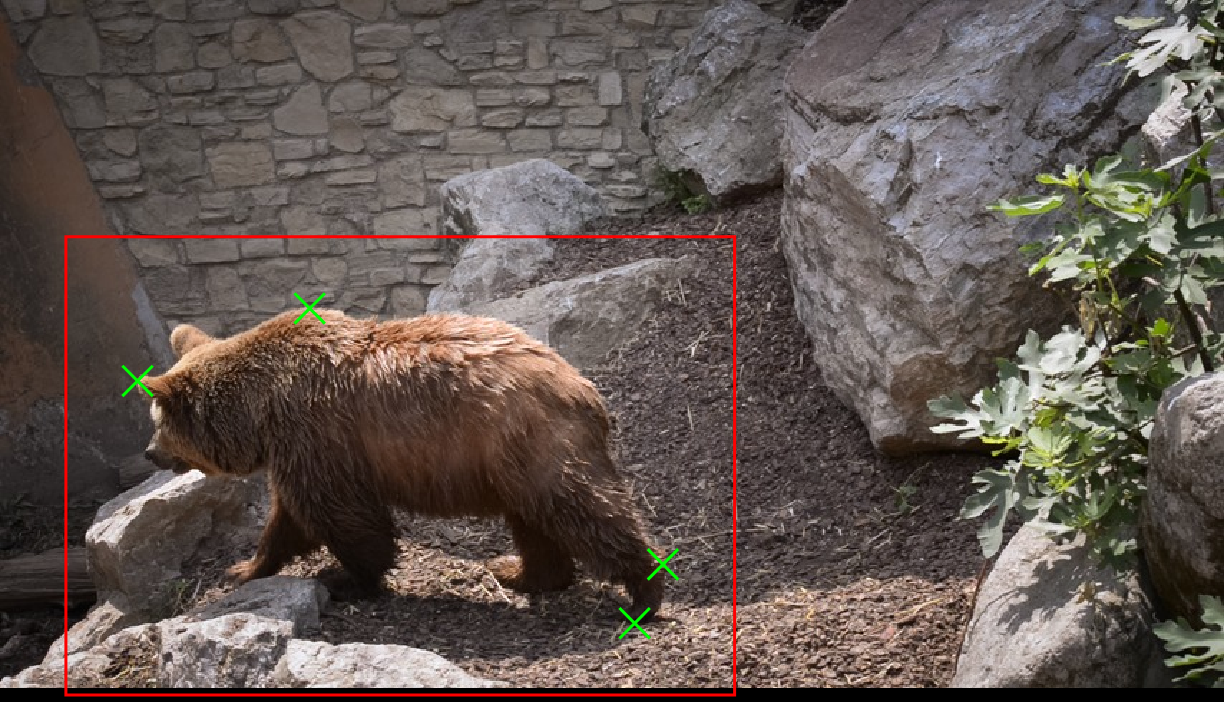
\includegraphics[width=\linewidth]{figures/chap33_bear_bbox.png}
	\caption[DEXTR User Interaction]{		
		Image with the obtained user input for the \gls{dextr} method and the first processing step.
		The extreme points are visualized as green crosses.
		The bounding box is enlarged by $p_{{box}} = 50$ \Unit{px}, shown in red.
		The enlarged bounding box extends the image boundary, therefore, \textit{zero padding} is applied.
		The corresponding cropped and resized image is shown in Figure \ref{fig:ch3:sec3:rgb_channel}.
	}
	\label{fig:ch3:sec3:user_interaction}
\end{figure}


% One feature map with extreme points
Second, the four extreme points are converted into one heatmap.
The points in this heatmap are located on the boundary of the object.

To highlight the extreme points a 2D Gaussian is centered around each point $ \textbf{p} (x_p, y_p) $ with the another points $ \mathbf{x} = (x, y) $ by
% Impelemtation in HDevelop:
% ResGauss := exp(-4 \cdot log(2) $\cdot$ ((Rows-PointRow)*(Rows-PointRow) + (Cols-PointCol)*(Cols-PointCol)) / (GaussSigma * GaussSigma))
\begin{equation} \label{equ:gauss}
	\centering
	Gauss \left( x,y \right)  = max \left( g\left( x,y\right) , \frac{\exp(- 4 \log_{2}(| \textbf{x} - \textbf{p} |_2)}{\sigma^{2}}\right) 
\end{equation}
where $ g (x,y) $ is the current grayvalue of the heatmap at position $ (x, y) $ and $ \sigma = 10 $ representing the standard deviation of the Gauss filter.
This heatmap is vital for the method, because of the high level guidance for the deep segmentation network.
A closeup of a point centered by the 2D Gaussian is visualized in Figure \ref{fig:ch3:sec3:gauss_centered_point}.

Third, the heatmap has the size of $512 \times 512$ \Unit{px} and is concatenated with the RGB image.
This results in the four-channel input for the \gls{dextr} model, illustrated in Figure \ref{fig:ch3:sec3:model_input_channels}.

\begin{figure}
	\centering
	\begin{subfigure}[t]{0.3\textwidth}
		\centering
		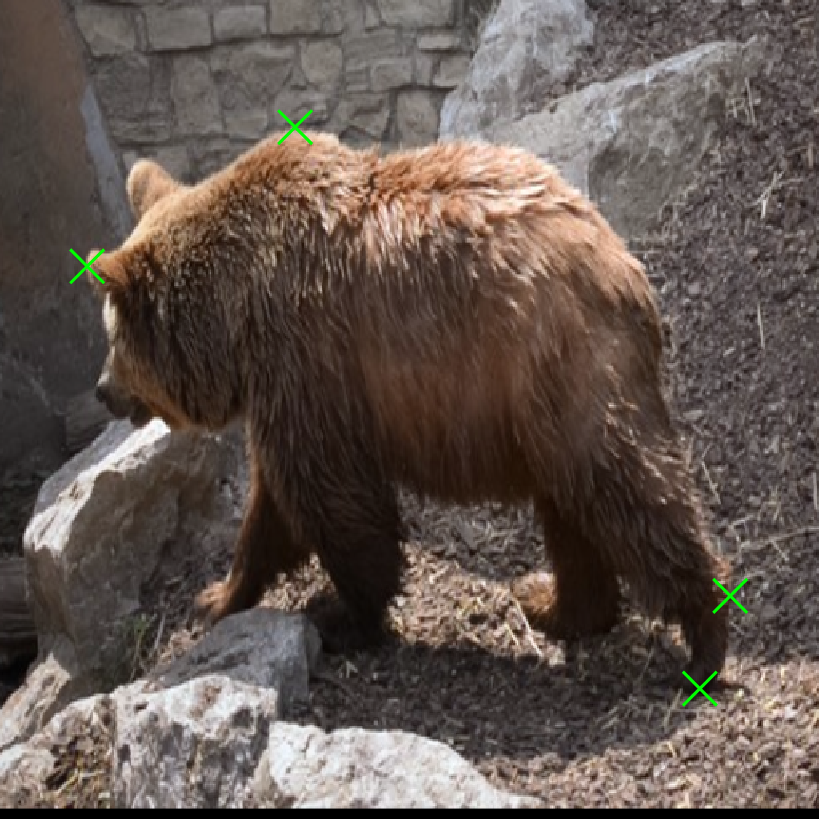
\includegraphics[width=\textwidth]{figures/chap33_channel_rgb.png}
		\caption{RGB image with the points cropped based on the bounding box (three channels).}
		\label{fig:ch3:sec3:rgb_channel}
	\end{subfigure}
	\hfill
	\begin{subfigure}[t]{0.3\textwidth}
		\centering
		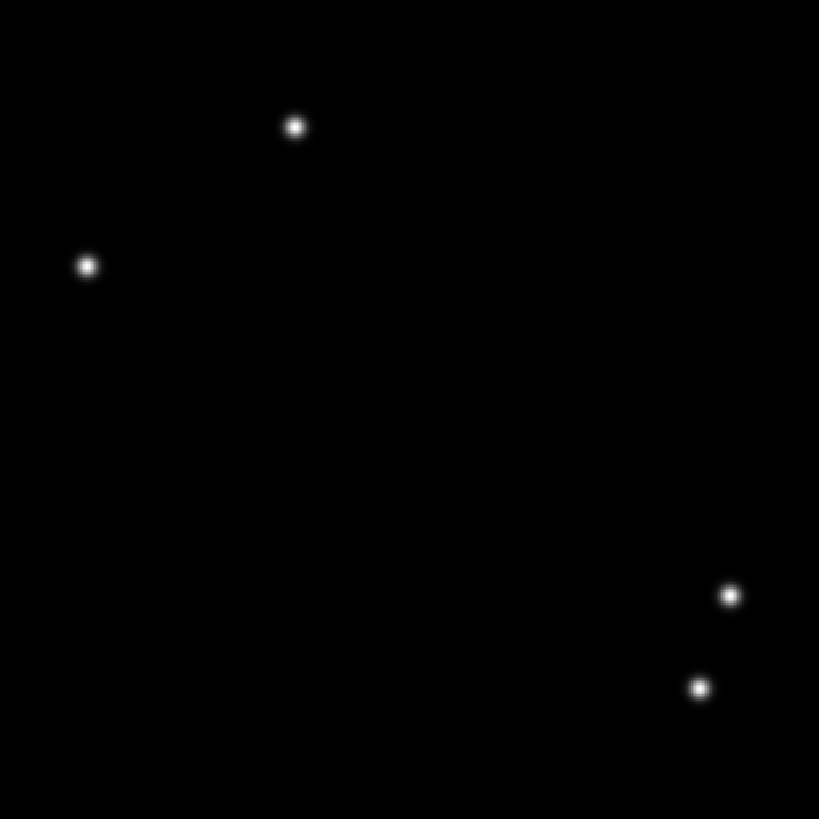
\includegraphics[width=\textwidth]{figures/chap33_channel_fg.png}
		\caption{Foreground heatmap with four extreme points (one channel).}
		\label{fig:ch3:sec3:fg_channel}
	\end{subfigure}
	\hfill
	\begin{subfigure}[t]{0.3\textwidth}
		\centering
		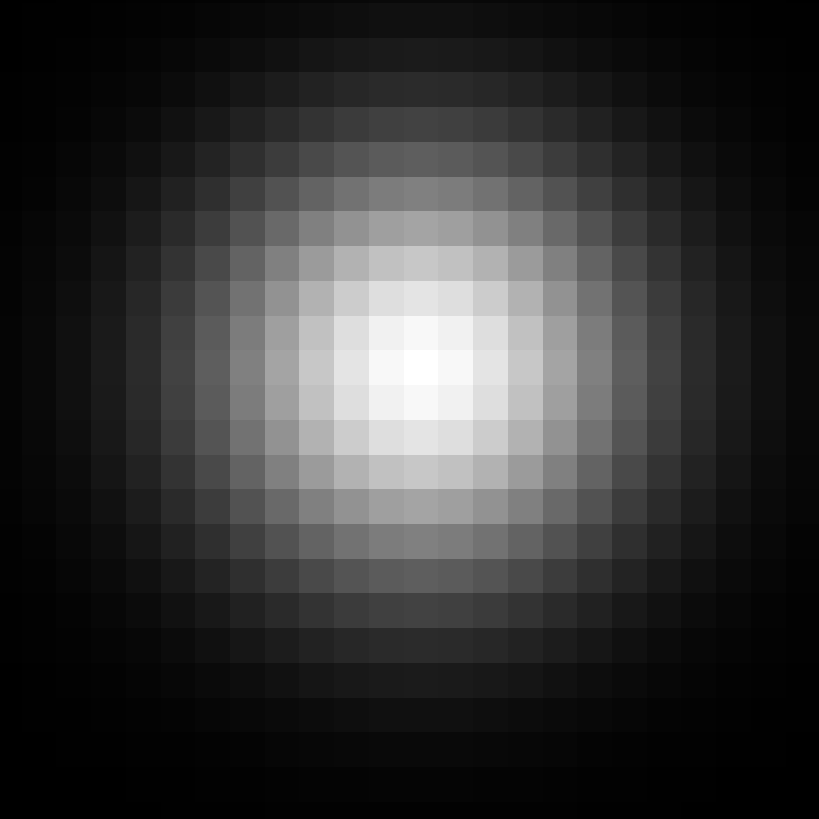
\includegraphics[width=\textwidth]{figures/chap33_gaussian_point.png}
		\caption{Closeup of a point centered with a 2D Gaussian with $\sigma = 10$.}
		\label{fig:ch3:sec3:gauss_centered_point}
	\end{subfigure}
	\caption[Four-channel DEXTR model input]{
		Representation of the separate channels from the four-channel input for the \gls{dextr} model.
		All channels have the spacial dimension of $512 \times 512$ \Unit{px}.
		The user points on the object's boundary are processed by the 2D Gaussian.
	} \label{fig:ch3:sec3:model_input_channels}
\end{figure}


\subsection{Architecture}\label{ord:ch3:sec3:subsec3}

As encoder for the segmentation network \textit{ResNet-101} \cite{He16-ResNet} is selected, which also referred to as \textit{backbone}.
The ResNet-101 is a deep \gls{cnn} containing 101 layers.
The core components of any ResNets are \textit{residual units}, whose main feature is the use of skip connections \cite{Ger17-HandsOn}.
The ResNet-101 is structured in four blocks, that each contain 3, 4, 23 and 3 bottleneck blocks.

The ResNet-101 used for \gls{dextr} is modified by including atrous convolution in the last two blocks and removing the fully connected layers.
After the backbone, a four staged \gls{psp} module is applied to preserve global context.
The decoder of this architecture does not consist of several convolution layers, instead bilinear interpolation is used to retrieve original spatial dimension of $512 \times 512$ \Unit{px}.
Finally, a sigmoid function is applied to obtain the final prediction $\textbf{y}$ as a  probability map. \footnote{Wolfram Math world, Sigmoid Function \url{https://mathworld.wolfram.com/SigmoidFunction.html}}

% Training settings.
The model is trained for $ n_{epochs} = 100 $ epochs on the PASCAL \gls{voc} 2012 Segmentation and further $ n_{epochs} = 10 $ epochs on the COCO dataset.
The learning rate is $ \lambda = 10^{-8} $ and the momentum is $ 0.9 $.


\subsection{Refinement}\label{ord:ch3:sec3:subsec4}

As introduced in Subsection \ref{ord:ch2:sec3:subsec2}, some interactive methods provide the possibility to perform refinement, if a segmentation result does not meet the user's expectations.
For the \gls{dextr} method the user may perform refinement by setting an additional click.
The refinement click should be located on the boundary of the region where the segmentation fails.
This new refinement click is added to the foreground heatmap with the extreme points.
In Figure \ref{fig:ch3:sec3:refinement} the effect of an additional refinement click is exemplary presented.
Each refinement click triggers a new model execution.
The refinement process may be applied iteratively.

% TODO plots use an example where the initial prediction actually fails and the refinement succeeds.
\begin{figure} [!b]
	\centering
	\begin{subfigure}[b]{0.45\textwidth}
		\centering
		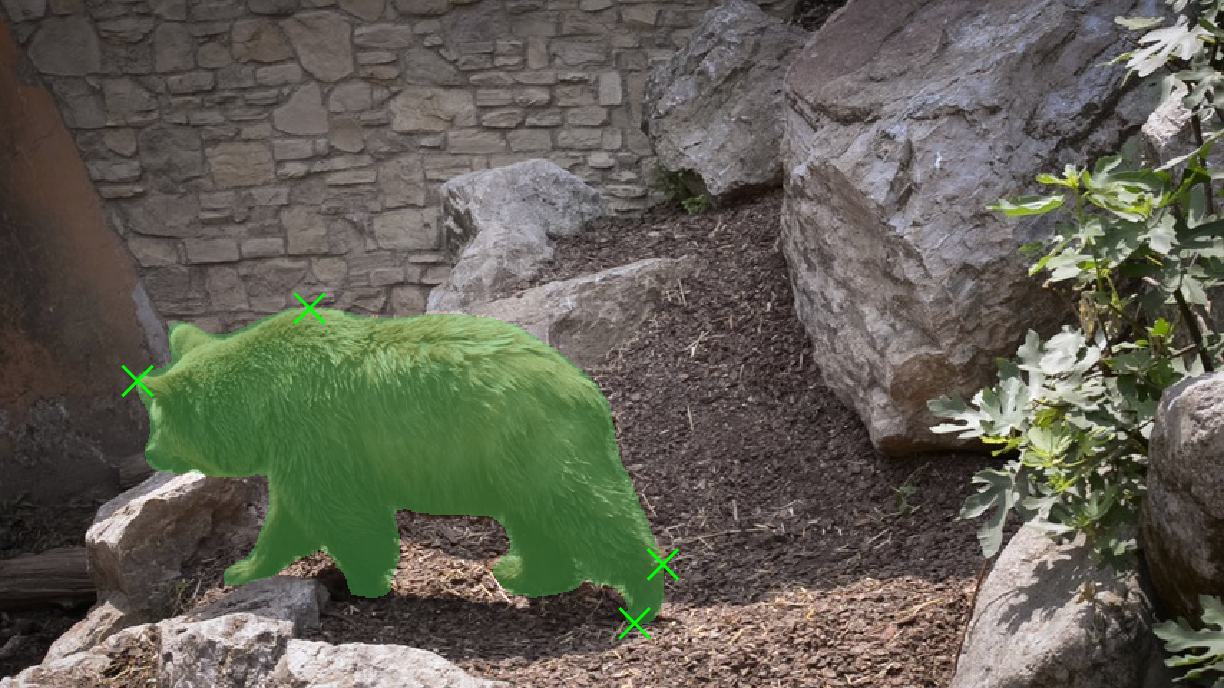
\includegraphics[width=\textwidth]{figures/chap33_bear_initial_result.png}
		\caption{Initial segmentation result.}
		\label{fig:ch3:sec3:refinement_1}
	\end{subfigure}
	\hfill
	\begin{subfigure}[b]{0.45\textwidth}
		\centering
		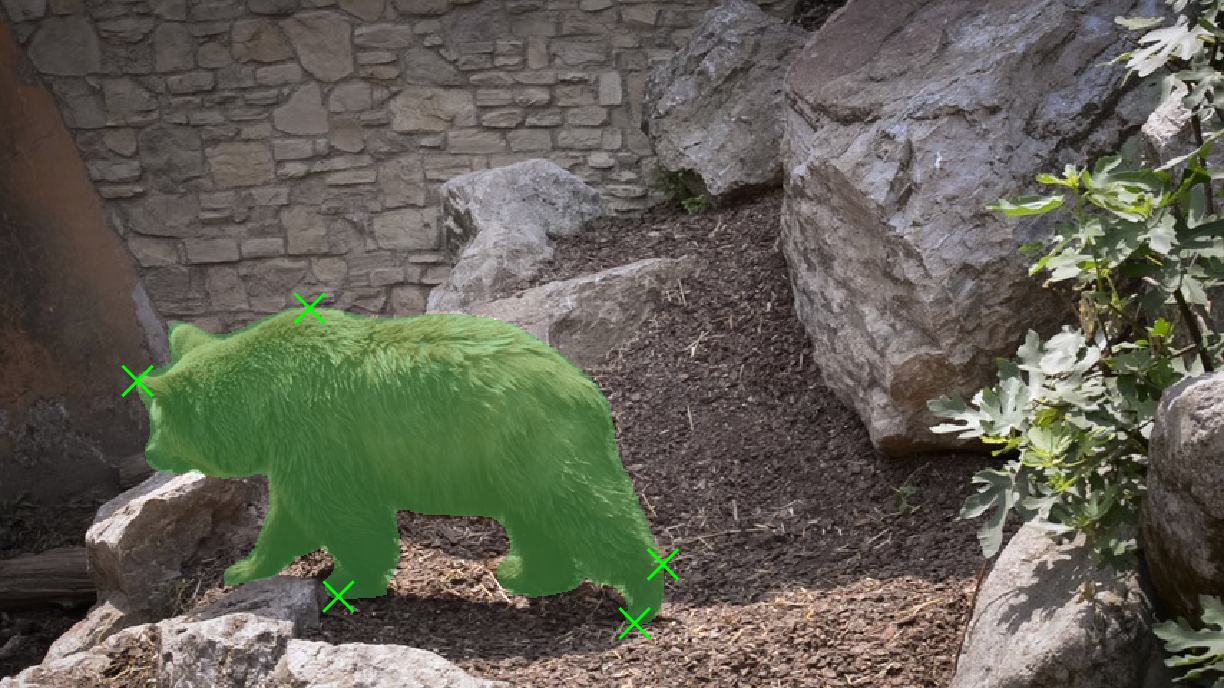
\includegraphics[width=\textwidth]{figures/chap33_bear_refine_result.png}
		\caption{Refinement segmentation result.}
		\label{fig:ch3:sec3:refinement_2}
	\end{subfigure}
	\caption[DEXTR Refinement]{
		On the left is the initial result with the normal extreme points. 
		On the right is the segmentation result with one additional refinement click.
	} \label{fig:ch3:sec3:refinement}
\end{figure}


\subsection{Performance}\label{ord:ch3:sec3:subsec5}

The performance of the \gls{dextr} method in comparison to other interactive segmentation methods in shown in Table \ref{tab:ch2:interactive-stae-of-the-art}.
In this comparison on PASCAL \gls{voc} the \gls{dextr} method performs well and is only outperformed by the \gls{iog} method.

The experiments and evaluations presented in \cite{Man18-DEXTR} contain various datasets and test settings.
Among them is also an examination of the performance on unseen classes and the generalization capability of the method.
Thereby, the model was trained with the PASCAL \gls{voc} or COCO dataset and evaluated on both datasets.
Despite these results seem reliable, it must be taken into account that the PASCAL \gls{voc} and COCO datasets are very similar and cover the same type of \textit{general} objects.
The evaluation of the generalization capabilities of the method continues in detail in Section \ref{ord:ch5:sec2_generalization_image_domains}.

An introduced application for the \gls{dextr} method is to create annotations and use them as new \gls{gt} to train \gls{dl} models.
Manisis \etal claim, that models trained on \gls{dextr} annotations perform equally well as models trained on the original \gls{gt}\cite{Man18-DEXTR}.
This statement is further examined in Section \ref{ord:ch5:sec5_retrain}.
Additional examples of segmentation results with the \gls{dextr} method are shown in Figure \ref{fig:appendix_model_predictions}.